
\chapter{Physics Object Reconstruction in CMS} \label{sec:cms_reco}

The excellent spatial resolution of the CMS trackers, high granularity of the calorimeters, and almost $4\pi$ coverage of the detector, allowed the CMS to introduce the particle flow (PF) algorithm \cite{Particle_flow} for a global event reconstruction. The PF takes the input from all subdetectors, analyzes the redundant information and removes the duplicate one. The PF procedure starts with identification of tracks and calorimeter clusters, then reconstructs the physics objects, such as muons, electrons, and jets. In this section, first we will discuss the tracking procedure, then the elements of the PF algorithm in greater detail will be described.
    
\section{Track Reconstruction}\label{sec:track_reconstruction}

The reconstruction starts with the clusters of signals (``hits'') in the inner tracker. The information from these clusters in the Pixel and Strip subdetectors is aggregated based on their signal-to-noise ratios. A charge-weighted averaging is performed (for different particle charge hypothesis). Then, a set of corrections is further applied to identify the real hit positions. 

Since the number of tracks at any given event can exceed O(100), a pattern recognition technique (PRT) is employed before any further reconstruction starts. The PRT identifies relevant tracks compatible with the candidates emerging from or near the IP. Then, the track reconstruction is applied to the selected set of tracks. 


The helix trajectory that a particle follows in the magnetic field inside of the detector is characterised by five parameters: the direction in $\eta$, the 3D position (of a particular point on the helix trajectory) with respect to the reference point, which is the center of the IP, and the curvature of the track (the inverse of the helix radius R). The radius of the trajectory is related to the momentum of the particle $p$ travelling in the magnetic field $B$ by the formula $R \approx p/B$. This information is enough to compute estimates of basic physics quantities; however, this task is complicated by the presence of high particle multiplicity in the event (the number of charged particles produced in the same event) and also by a physics aspect of the electron propagation in matter: an electron traversing the detector has nearly 85 $\%$ probability to emit a bremsstrahlung photon. Hadronic effects also need to be taken into account; a hadron has a 20$\%$ probability to experience multiple scattering on the nuclei of the detector before reaching the HCAL. 



To keep the track finding efficiency high, while maintaining low efficiency of misidentified tracks, track reconstruction is performed sequentially using the combinatorial track finder (CTF) \cite{combined_track_finding}, see Fig. \ref{ctf}. First the "purest" tracks are reconstructed; they have high $p_T$ and the hits of the particle candidate point towards the beam spot. Then the hits associated with these pure tracks are removed from the collection of considered hits and another round of the track reconstruction starts. Applying this procedure several times reduces the combinatorial factor and also simplifies the identification of tracks with low $p_T$ or those which do not point to the beam spot. During each iteration, the reconstruction follows these steps:


 \begin{figure}[H]
  \centering
  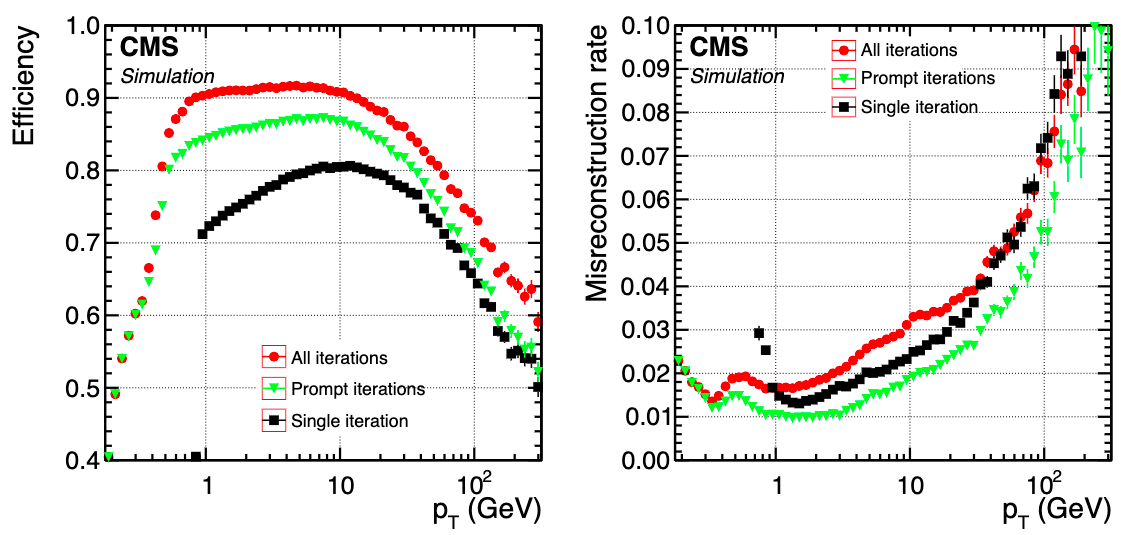
\includegraphics[width=0.96\textwidth]{ctf}
  \caption[Global combinatorial track finder efficiencies. ]{Global combinatorial track finder efficiencies as a function of the track $p_T$. Left: signal efficiency. Right:  misidentification rate. Single iteration of the CMT is shown using black squares. The iterative tracking method consisting of 10 iterations is shown using green triangles and red circles. Prompt iterations based on seeds with at least one hit in the pixel detector are shown in green. All iterations are shown in red, including iterations when displaced seeds are present \cite{PFalgo}.  }\label{ctf}
\end{figure}


\begin{itemize}
\item Seed generation. Rough estimates of the particle trajectories ("seeds") are produced using either three hits or two hits and a beam spot constraint. Based on which iteration the algorithm is on, some additional constraints are applied, e.g., a minimal $p_T$ selection, the requirement for the seed to originate close to the beam spot, etc. 
\item Trajectory building. Initial seeds are projected towards the compatible hits in the next layers. This approach is based on the Kalman Filter (KF) procedure \cite{Kalman_filter}. The extrapolation is done until the outermost layer of the tracker is reached or when a "terminating condition" is satisfied, e.g., when the iteration accumulated the maximum allowed number of invalid hits ("fake hits"). Each obtained trajectory is updated using a KF approach based on the compatibility of hits to form a better track candidate. The procedure is complicated by the fact that the same initial seed can give rise to several track candidates or vice versa, the same track candidate may be compatible with different seeds. Additionally, the trajectory building step should take into account energy loses of the particle due to multiple scattering on the detector material, inhomogeneities of the tracker material, and the effects of the regions of nonconstant magnetic field. 
\item Track fitting. After the track candidate has been built, the track parameters are refitted by a KF and by the "smoother". This step uses the full available information about the track and gives optimal estimates of the track parameters. To remove a large number of fake tracks, which are present due to a  complicated nature of the problem and the high track multiplicity in the event, a multivariate (MVA) selection is applied. The MVA discriminant incorporates variables that discriminate real tracks from the fakes: the signed transverse curvature and impact parameters (with respect to the beam spot), the polar and azimuthal angles, number of missing hits, the fit quality variables, etc. 
\end{itemize}

The CTF procedure runs for 10 iterations. In 2016, the proton-proton collisions had a mean pileup (PU or additional hard scattering vertices) of 24, the CTF efficiency to identify real tracks varied from 80 to 95$\%$ with the mis-identification efficiency of 5 - 10 $\%$ depending on the $p_T$ and $\eta$ of the tracks.

\subsection{Muon tracking}\label{sec:muon_track_reconstruction}

Muons are detected not only by the inner tracker but also by the outer (muon) tracker. This greatly improves muon track reconstruction, in comparison to using just the inner tracker information. Also, it motivated the development of dedicated muon reconstruction algorithms. Therefore, the ninth and the tenth iterations of the CTF are focused on the muon reconstruction. These iterations use three separate algorithms to identify: 

\begin{itemize}
\item Standalone muons. This algorithm uses only muon tracker information: DTs, CSCs, RPCs. Hits from the inner chambers are used as seeds and are projected to hits in the outer chambers. Then, a standard KF procedure is used to identify track candidates, which are called standalone muons.
\item Tracker muons. Only the inner tracking information is used to form tracks. Tracks are further projected to muon subsystems, where a compatibility with at least one muon hit is required. This algorithm works with low momentum muons: tracks with $p_T$ above 0.5 GeV and a total momentum greater than 2.5 GeV.
\item Global muons. Tracker tracks and standalone tracks are projected to the outermost layer of the muon system, checking the compatibility between two approaches. The resulting combined set of track hits is refitted to produce a global muon track. Mostly high momentum muons with $p_T > $ 200 GeV profit from this algorithm.
\end{itemize}

\subsection{Electron tracking}\label{sec:ele_track_reconstruction}
Electrons are also detected by the inner tracker. However, their reconstruction is complicated by the fact that they emit bremsstrahlung photons and the trajectory becomes more complex. As a result, the clustering algorithms also need to identify the bremsstrahlung photons and account for the fact that the energy clusters corresponding to these photons may be located outside of the main electron trajectory when extrapolated to the ECAL. 

In the KF approach, it is assumed that energy losses are Gaussian, and this is not the case for electron. A dedicated procedure is developed - a modified KF - the Gaussian Sum Filter (GSF) \cite{GSF}. In this method, the radiated energy losses are approximated by the sum of weighted Gaussian distributions. 

The electron seeds for the GSF are built using the ECAL information. Two different approaches are developed for the track reconstruction:

\begin{itemize}

\item Super Cluster based electrons. Clusters of energy in the ECAL are grouped together to form super clusters (SCs). Using the information of the energy spread among the clusters, the curvature of the electron's path is estimated and tracker seeds are formed, using the SC position as a constraint. 
\item Track based electrons. Tracks from the inner tracker are projected to ECAL clusters, checking the compatibility using quality variables, such as $\chi^2$, number of missing hits (absent hits along the path of the track), etc. 
\end{itemize}

A typical momentum resolution for electrons in $Z \rightarrow e^- e^+$ decays is in the range of 1.7 - 4.5$\%$.

\subsection{Primary Vertex reconstruction}\label{sec:PV_reconstruction}

At the level of the LHC luminosity, several hard scattering vertices are produced in each collision. The location of these vertices is reconstructed using the tracks. However, normally only the primary vertex (PV) of these vertices produces interesting physics interactions and is the actual point of origin of the produced prompt particle. Other vertices are referred to as additional vertices or PU. 

All the vertices are important because they are reused in the feedback loop of the track reconstruction procedure. Furthermore, a precise identification of primary vertices is important for determining the effect of the PU on all physics objects in general and b-tagging in particular (this will be discussed later in this chapter). The PV identification consists of three steps: the tracks are selected, then the tracks from the same PV are combined in clusters, and, finally, the position of the PV is determined from the fits to tracks. 

When selecting the tracks, only those consistent with the locations of the hard scattering vertices are considered. Three variables are used to improve the quality of the track selection procedure: the transverse impact parameter (the relative distance in the vertical plane with respect to the center of the beam spot), the number of strip and pixel hits associated with a track, and the $\chi^2$ of the fit.

Clustering of the tracks is based on their z position in conjunction with the beam spot. A deterministic annealing (DA) algorithm \cite{DeterministicAnnealing} is used to find the global minimum for this problem with many degrees of freedom. The idea of this algorithm is based on the thermodynamic system in physics, approaching a state of minimal energy through a series of temperature reductions. 

Once the clustering is completed and hard scattering vertices are identified, the candidates with more than two tracks are fitted using an adaptive vertex fitter \cite{AdaptiveVertexFitting}. The result of this procedure is a set of probabilities assigned to tracks. Each probability can be conceptualized as the likelihood that the track originated from a given vertex.

At the final stage, the vertices are ordered by the sum of the squared transverse momenta ($\sum p_T^2$) of the corresponding tracks and the vertex with the largest value of the $\sum p_T^2$ is called the main hard scattering vertex, or the PV. The resolution of the PV varies between 10 to 100 $\mu$m and depends on track qualities. 

\section{Particle level objects}\label{sec:pf_objects}
\subsection{Particle Flow links and blocks}\label{sec:some_reconstruction}

The signals a particle leaves (in several CMS subdetectors) are stored as PF \cite{ParticleFlow} elements. The link algorithm (LA) was developed to connect these PF elements. The LA can test any pair of elements in the event. To speed up the calculations, only pairs of elements that are "neighbors" in the given $\eta - \varphi$ plane are considered. When the pair of elements are linked, the LA determines the distance measure between the elements which is related to the quality of the link. This procedure produces PF blocks of elements, where the blocks are connected either by a direct or an indirect link (through the common elements).

The procedure produces inner tracker-calorimeter, HCAL-ECAL, ECAL-ECAL  cluster-to-cluster, and ECAL-Preshower links. In most cases the link distance is defined in the $\eta-\varphi$ or $x-y$ planes between the two cluster positions. In case of the ambiguity when, e.g., several HCAL clusters are linked to the same ECAL cluster, only one link is kept, the one with the smallest distance.

The last stage of the link algorithm is dedicated to formation of the inner tracker-muon system links. Once all links are established and PF blocks are formed, the PF algorithm proceeds reconstructing objects in a specific sequence. Muon candidates with corresponding PF tracks and clusters are reconstructed and then removed from the PF block. After that electron candidates with the identified bremsstrahlung photons, and high momentum isolated photons with related tracks and clusters are reconstructed and removed, in that order. Finally, charged hadrons and non-isolated photons are processed.

The elements that are still left in the PF blocks are then re-considered for another round of identification of other objects: charged hadrons and neutral hadrons, photons from parton fragmentation and hadronization, and jet decays. Lastly, when all PF blocks have been sorted and identified, the global event description is completed and the reconstructed event is re-processed by a post-processing step (PP step), addressing the possible particle misidentification and improper reconstruction during the previous steps. 

\subsection{Muons}\label{sec:muons}

Muon reconstruction is the first stage of the PF algorithm. It identifies muons using global and inner tracker muon properties. Global muon candidates are selected at this step and the isolation requirement (explained later in this chapter) is applied. This isolation requirement is efficient enough to reject hadrons mis-identified as muons. The muons inside jets or secondary muons from hadron decays complicate the identification of prompt muons, such as those originating from Higgs, W, or Z boson decays. Therefore, an additional more stringent selection is further applied. 

For non-isolated global muons, in addition to the Tight Working Point (WP) selection (a set of requirements to remove fake muons), the following extra selection is applied: more than two matching track segments should be present in the muon detectors or the calorimeter energy deposits must be compatible with the energy of the muon candidate. This selection discriminates against high $p_T$ hadrons. If muons fail Tight WP, there are additional recovery procedures that use the relaxed selection criteria to search for lower quality muons.

Even at this stage in the PF procedure, the muon identification and reconstruction is not finished. Charged hadrons reconstructed during the next PF stages can be reconsidered as muon candidates. Only after the whole PF sequence is completed, including the PP step, the PF procedure is completed.

All muons considered for this measurement are global muons that satisfy the Tight WP requirements (as an initial selection) with extra requirements on the number of hits in the tracker and muon system, on the impact parameter, and the quality of the global track. 

The efficiency $\epsilon$ to successfully identify a prompt isolated lepton can be decomposed as:

$\epsilon = \epsilon_{tracker} \cdot \epsilon_{ID | tracker} \cdot \epsilon_{ISO | ID} $

\noindent where the first term refers to the tracker efficiency, the next term is the Bayesian term which refers to the identification (ID) efficiency given that the lepton already passed the tracker requirements, and the final term refers to the isolation (ISO) efficiency given that the lepton already satisfied identification criteria. All the efficiencies are well optimised in the CMS and are in the range from 85 $\%$ to more than 99 $\%$ depending on the $p_T$ and $\eta$ of the lepton (muon in this case). The muon momentum resolution for 20 to 100 GeV momentum range varies from 1 $\%$ in barrel to 5 $\%$ in endcaps.

\subsection{Electrons and isolated photons}\label{sec:electrons}

The reconstruction of electrons is complicated by the fact that they lose energy emitting bremsstrahlung photons and, thus, their trajectory becomes more complex than the one of muons. Additionally, bremsstrahlung photons often convert to $e^+ e^-$ pairs. This is a recursive process, as daughter electrons also emit photons. Due to this complication, it was decided to use almost the same procedure to reconstruct electrons and photons. First a GSF track plays a role of the seed for the electron candidate. For the photon candidate, an ECAL supercluster with no links to the GSF track is used as a seed. For both electron and photon candidates energy deposits in the HCAL must not exceed 10$\%$ of the ECAL energy. 

ECAL energy deposits, that are above a certain threshold and close to the most energetic deposit, are then grouped into the SC and may be linked to one of the GSF track candidates. The energy of the collected ECAL energy deposits is corrected for the additional energy losses during the linking procedure. An electron candidate is formed from a combination of the corrected ECAL energy and the electron direction given by the GSF track. An additional MVA discriminator of O(20) variables is applied to improve electron identification efficiency. The MVA approach, based on the Boosted Decision Trees (BDT) classifier \cite{TMVA}, profits from the following highly discriminating variables: the amount of energy radiated off the GSF track, the distances between the ECAL SC position and the position given by the tangent to the GSF track, track-cluster linking variables, KF and GSF track quality variables, etc. 

Photon candidates are kept if the photons are isolated and the corresponding configuration of ECAL energy deposits is compatible with those expected from a given photon shower.  All identified electron and photon tracks and clusters in the PF block are masked before the algorithm starts processing hadrons. 

As offline physics analyses apply different selection for electrons and photons, PF selection is relatively loose and  the full electron and photon reconstruction information is saved in case a different re-interpretation must be run. This offers the saving of the computing time in the future, since re-running the electron track reconstruction would not require re-running the complete PF algorithm again.

\subsection{Hadrons and non-isolated photons}\label{sec:hadrons}

After the muons, electrons, and isolated photons are reconstructed, they are removed from the PF blocks. The next PF algorithm iterations proceed with hadrons from jet fragmentation and hadronization. These particles can be ``seen'' by the detector as charged pions, kaons or protons, neutral pions and kaons, and non-isolated photons from neutral pion decays. During the reconstruction, precedence is given in the ECAL to photons over neutral hadrons. This priority does not hold above $|\eta| > 2.5$. In that region, ECAL clusters linked to a given HCAL cluster are identified as hadrons and, only if ECAL clusters are without such a link, then they are classified as photons.  

What is left in the PF block may be considered a neutral hadron if there are ``absent'' tracks in the tracker. If tracks are present and compatible with the  energy deposits, a charged pion candidate is formed. 

In situations where the energy deposits in the calorimeters do not match the energy hypothesis from the tracker well, and this discrepancy is larger than three standard deviations, a new muon reconstruction starts, with the relaxed muon selection. This approach allows to improve the muon identification efficiency without increasing the rate of mis-identified muons. 

At times the energy associated with the track momentum sum may be found to be significantly larger than the calorimetric energy. Usually this excess in momentum is found to arise from residual mis-reconstructed tracks with a $p_T$ larger than 1 GeV. These tracks are sorted in decreasing order of their $p_T$ and are removed one-by-one from the PF block until no such tracks are left in the initial track collection.

The hadron traversing the material of the tracker interacts with the nuclei of the tracker material and often produces secondary hadrons. These secondary hadrons are produced outside of the PV - at a secondary (intermediate) interaction vertex. When the tracks of the charged particles corresponding to these secondary particles are linked together, the resulting secondary particle candidates can be  replaced in the list of reconstructed particles by a single (original) charged hadron.  

The estimate of the energy of the primary charged hadron is then given by:

$E = E_{secondary} + f \cdot p_{primary}$

\noindent where $E_{secondary}$ is the vectorial sum of the momenta of the secondary charged particles, $p_{primary}$ is the momentum of the incoming track, and $f$ is a factor determined from the simulations. 

\subsection{Jets and jet corrections}\label{sec:jets}

Jets are collimated streams of particles created during the processes of the fragmentation and hadronization of the original parton, quark, or gluon. As jets propagate through the CMS detector, they leave tracks in the tracking system and interaction showers in the calorimeter crystals. 

Several jet reconstruction algorithms have been developed. In the Higgs boson group of the CMS, most measurements are using anti-$k_T$ algorithm \cite{antiKt}. If the jet clustering uses PF particles, then PF jets are reconstructed. If only the ECAL and HCAL information is used, calorimeter jets are identified ("calo jets"). When all stable particles (in case of the simulation, at the generator level) excluding neutrinos are used - reference jets are reconstructed ("Ref jets"). In this measurement PF anti-$k_T$ jets are used. 

The anti-$k_T$ algorithm is one of the ``cone'' algorithms that takes as input a collection of PF objects inside of a cone of the radius R, which is the parameter that determines the final size of the jet and is usually between 0.4 - 0.7. The algorithm defines the distance parameter
$d_{ij} = \min (\frac{1}{p^2_{T_i}}, \frac{1}{p^2_{T_j}}) \times \frac{R^2_{ij}}{R}$, where $p_{T_i}$ and $p_{T_j}$ refer to the transverse momenta of PF particles $i$ and $j$, $R_{ij}$ is the distance in the $\eta - \varphi$ plane between particles $i$ and $j$. An additional $d_{iB}$ parameter is defined as the distance between the particle $i$ and the beam spot position: $d_{iB} = \frac{1}{p^2_{Ti} }$.

This algorithm iteratively finds the minimum distance selecting at each step the minimal value for each ($d_{ij}$, $d_{iB}$) pair, using a collection of the PF particles as an input. The algorithm then seeks out the smallest $d$ for a given input. If the minimum distance is $d_{ij}$, then the four-vectors of $i$ and $j$ particles are summed to form a new particle. Particles $i$ and $j$ are removed from the initial input collection. If the minimum distance is $d_{iB}$, then the particle $i$ (a PF particle candidate) is considered a jet. This particle is also removed from the set of particles and the algorithm continues until all initial particles have been combined into jets. The mechanics of the algorithm is such that first jet candidates with the hardest particles are clustered, producing a perfect cone-shaped jets, then more complex jets are reconstructed.

PF jets were used to conduct the data analysis in this thesis. They are superior to calo jets because the former have a better angular resolution. The PF algorithm allows the precise determination of the charged hadron direction and momentum, while in calorimeters, the energy deposits of charged hadrons are spread along the $\varphi$ direction in the presence of the magnetic field, which leads to an extra degradation of the azimuthal angular resolution of jets.

On average, the relative contributions to jet energy are: 65$\%$ from charged hadrons, 25$\%$ from photons, and 10$\%$ from neutral hadrons. The possibility to identify the contributors to the total jet energy during the jet reconstruction is one of the reasons to use the PF algorithm for jet reconstruction. In practice, the identification of particles inside jets is done by comparing the jet energy fractions measured in PF jets to those of the corresponding Ref jets.

To remove the jet energy dependence on p$_T$ and $\eta$ (JE map), and make the corresponding two dimensional JE map uniform, the jet energy correction (JEC) procedure is introduced. The jet energy resolution (JER) correction is also necessary. The latter is defined as the Gaussian width of the ratio of the energies of the corrected PF jets to Ref jets. Both corrections improve the angular resolution, energy response, energy resolution of jets, and make the simulation match the data. 

The JEC scales the four-momentum of jets. Various detector effects are addressed. This correction is often split into separate components, which are applied individually in a sequence. The most important individual corrections remove energy contributions due to PU, effects of the calorimeter response, residual data-Monte Carlo (MC) discrepancies, and effects of the jet flavor.

JER smears the four-momenta of reconstructed jets to match the energy resolution observed in data. The smearing procedure derives the correction factors which scale the momentum of the reconstructed jet with respect to the the momentum of the ``gen'' jet, which is same jet, but clustered at the MC generator level.

\section{Other important physics quantities and objects}
\subsection{The b tagging and secondary vertices}\label{sec:btag}

In this measurement, one of the Higgs bosons will decay into b quarks. Jets produced during the hadronization of b quarks are called b jets. A dedicated b tagging is necessary since \HBB~decay has the highest branching fraction of almost 58$\%$. Therefore, measuring precisely this BF is a great test of the SM.

Bottom quarks will produce jets that contain B mesons (or some baryons containing a b quark), which have a relatively long lifetime $c \tau \approx 500 \mu$m. This distance, traveled at almost the light speed, would correspond to a dislocation of a few mm from the PV. The positions of B meson decays will be clearly seen in the detector. Each such position with a corresponding displaced vertex, the secondary vertex (SV), is a unique signature of b quark and is used to identify the b quark decay. Sometimes the vertex cannot be unambiguously reconstructed, but even in these cases the properties of tracks within b jets are different from the ones originating from gluons or light quarks (light jets).

After passing the selection criteria, tracks are considered for b tagging. The selection requirements, which include kinematic and impact parameter properties of tracks, are needed to reject fake tracks, tracks coming from PU vertices, and tracks from the long-lived hadrons. 

Two main approaches are used to reconstruct the secondary vertices (SV). One of the methods that pioneered the b tagging is an adaptive vertex reconstruction (AVR) algorithm. AVR is based on the adaptive vertex fitter; it uses the tracks associated with jets and finds PV and SVs. The other algorithm is the inclusive vertex finder (IVF). IVF uses all the tracks in the event and is implemented with the selection looser than for the AVR. 

As for the b tagging itself \cite{CMS-PAS-BTV-15-001, Sirunyan:2017ezt}, multiple algorithms (taggers) have been developed and successfully used over the last decades. The most known ones are: 

\begin{itemize}
\item the jet probability (JP) and the jet b probability (JBP) taggers. Both are based on the probability of a jet candidate to be compatible (or incompatible) with the PV using impact parameter significance (IPS) variables.
\item The soft electron tagger (SET) and soft muon tagger (SMT). These taggers are based on the presence of soft leptons within jets, focusing on leptonic decays of B hadrons, because B hadrons have a larger BF to leptons than other hadrons do.
\item The combined secondary vertex (CSVv2) tagger. This is a more complex tagger based on an MVA technique. It uses displaced tracks and secondary vertices to tag b jets and takes as input IPS, decay length, SV parameters, number of SVs, etc. This tagger can use both AVR and IVF vertices.
\end{itemize}

In this physics analysis a new MVA based tagger (cMVAv2) was used. This superior tagger uses the outputs from all the aforementioned "fundamental" taggers: JP and JBP, SET and SMT, CSVv2 using both AVR and IVF vertices. These ensemble learning procedure \cite{ensemble_learning} of combining outputs from fundamental taggers into one complex MVA based tagger that produces the final output is a popular machine learning technique that has been proven to lead to better results than the ones achieved by individual algorithms separately. 

\subsection{Missing transverse momentum}\label{sec:met}

When neutrinos are present in the event, they cannot be directly detected by the CMS; specific neutrino detectors would be needed in this case. However, using the CMS detector one can indirectly estimate the momentum of neutrinos. This procedure relies on the method of the ``missing  transverse momentum`` \PTslash (or missing transverse energy  \ETslash (MET)), see Fig. \ref{missing_momentum}.  MET is constructed using all PF particles in the event and is calculated as:

$\PTslash = \vec{p}^{miss}_T = |- \sum^N_i \vec{p_{Ti}} |$. 




 \begin{figure}[H]
  \centering
  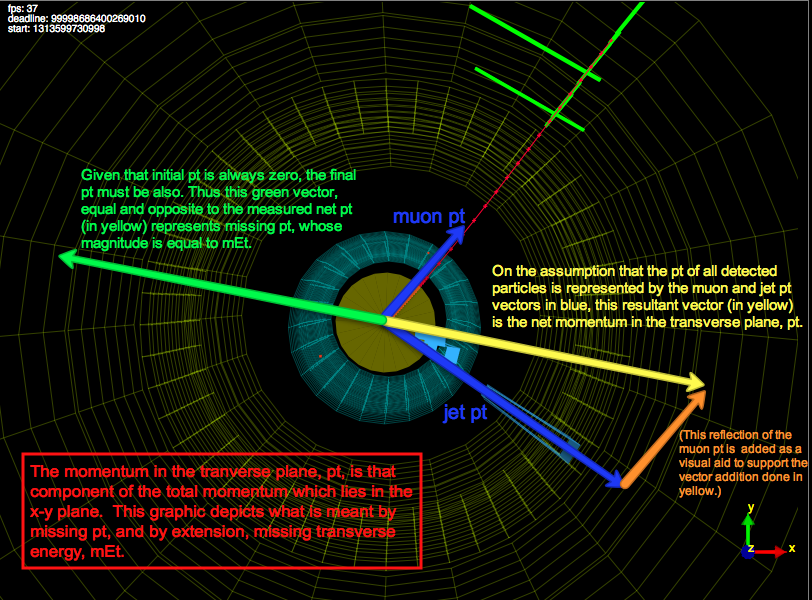
\includegraphics[width=0.9\textwidth]{missing_momentum}
  \caption[MET reconstruction in the CMS.]{MET reconstruction in the CMS. The only detected (visible) particles are muon and jet both shown using blue arrows. The total net momentum ``seen'' by the CMS detector is represented by the yellow arrow. From the conservation of momentum, the reconstructed MET corresponds to the green arrow. Taken from \cite{missing_momentum}. }
  \label{missing_momentum}
\end{figure}





To reconstruct $\PTslash$, the CMS relies on almost $4 \pi$ coverage of the detector and precise measurement of the particle properties using PF algorithm that takes information from all subsystems. The resulting $\PTslash$ is still considered "raw", since this MET is not yet JEC or JER corrected. After these corrections are applied, one obtains  $\PTslash$ that is called "Type-1 corrected MET". This is the version of MET that is recommended by the CMS JetMET particle Object Group (POG) group and is used in this measurement. An additional set of filters and corrections is further applied to reject events with artificially large $\PTslash$ due to the presence of several noise sources, such as ECAL dead cells, poor quality muon candidates, and HCAL noise. 

\subsection{Pileup interactions}\label{sec:pileup}

In 2016, a typical collision event contained on average 24 interaction vertices. Some events had nearly 40 inelastic proton-proton interactions. All the vertices excluding the PV can be referred to as the soft vertices. These soft vertices or PU do not produce interesting physics interactions, however, they contribute considerably to the total number of particles produced in the event. PU creates additional hadrons and photons and this affects the PF reconstruction of jets and $\PTslash$, and also the lepton isolation calculation.

Charged hadrons which have originated from PU are identified by backtracking the origin of the tracks and checking the compatibility with the PU vertices. These charged hadrons are removed from the collection of particles used to reconstruct physics objects. This procedure is called the charged-hadron subtraction (CHS). Because neutral hadrons and photons leave no tracks in the inner tracker, their presence needs to be identified and addressed differently. Instead, an average density $\rho$ of PU interactions in the given $\eta - \varphi$ slice is calculated. Assigning the area of the candidate to the value $A_{eff}$ ("effective area"), the expected PU initiated contribution that needs to be subtracted, is calculated as $\rho \cdot A$. Several other techniques are available, with one of the most simple relying on the calculation of the ratio of the neutral to the charged energy coming from PU (around a given lepton). From the studies, this value (called $\Delta \beta$) is determined to be very close to 0.5 \cite{PU_mitigation}. 

\subsection{Lepton isolation}\label{sec:isolation}

As mentioned before, lepton isolation is the preferred method to remove clear fakes and select real  prompt  muons  and  electrons  produced  by Higgs boson decay or by the weak decays of Z or W bosons. The isolation quantifies the activity of other particles around the particle of interest. The lepton isolation is defined as the scalar sum of the $p_T$'s of all charged and neutral hadrons and photons inside a cone of the radius $\Delta R <  0.3 - 0.4 $(depending on the WP and a lepton flavor). The sum is normalised by the $p_T$ of the lepton of interest:

$I_{PF} = \frac{1}{p_{T_\ell}} (\sum^\gamma p^\gamma_T + \sum^{h \pm} p^{h \pm}_T + \sum^{h^0} p^{h^0 }_T)$

There are other physics analysis-specific definitions of isolation and they are applied offline. For the purpose of this thesis, the two isolation requirements listed below are used.

For electrons, the isolation selection relies on the notion of the effective area defined in the previous subsection. The effective areas are proportional to $\Delta R$ cone size around the electron (0.3 in this case), and for electrons the isolation is given by: 

$I^{electron}_{PF} = \sum^{h^\pm} p_T + max (0, \sum^{h^0} p_T + \sum^\gamma p_T - \rho \cdot A_{eff})$.

The $\Delta\beta$ method mentioned previously is used for muon isolation selection. With the cone size of 0.4, the isolation is given by:

$I^{muon}_{PF} = \sum^{h^\pm} p_T + max (0, \sum^{h^0} p_T + \sum^\gamma p_T - \Delta \beta  \cdot  \sum^{h^\pm_{PU}} p_T)$.

\noindent The last term is the $\Delta \beta$ correction multiplied by the sum of $p_T$'s of the charged hadrons originated due to PU.

Both isolations are constructed from the collection of particles containing charged and neutral hadrons, photons, and charged hadrons from the PU (in case of muons).


\subsection{Data-Monte Carlo corrections}\label{sec:data_mc}

Even though particle interactions in the detector, the detector response, and the work of subsystems are simulated at a level of high precision, there is still disagreement present between the data and the simulation. The approximations used to speed up the subsystem responses, slight detector misalignments, the impossibility to know the exact parton distribution function (PDF) of the interacting particles at the interaction vertex, fluctuation of the LHC parameters and other factors contribute to the data-MC discrepancy. To reduce this disagreement, corrections factors are introduced. Efficiencies of different selections are measured both in data and in the MC, and their ratio is applied to the MC to make the MC similar to observed data. These ratios (corrections), also called ``scale factors'' (SF), are derived for all physics objects and the most important ones are discussed below.

\subsubsection{Lepton efficiencies and the Tag-and-Probe method}\label{sec:TnP}

Several steps are involved in the process of selecting a prompt lepton: tracking, identification, isolation, and trigger stages. A popular technique to measure the efficiency of these stages is called the Tag-and-Probe ($T\&P$ or TnP) method. Decays of $Z \rightarrow e^- e^+$ or $Z \rightarrow \mu^- \mu^+$ are used in this technique. The procedure first picks one lepton that has to pass a relatively tight ID selection; this lepton is called the ``tag''. Tags are often referred to as ``golden'' electrons or muons and have a low fake rate of the order of 1$\%$ or less. Then the other lepton, called the ``probe'', is selected to make a pair with the tag. This step results in total of $P_{total}$ pairs. This pairing procedure includes some very basic selection:  probes should be of the opposite sign and the same lepton flavor (OSSF). We need an unbiased source of leptons, and Z boson decay is a good source of such leptons. Therefore, the consistency with the Z boson pole mass is further checked. The exact definition of the probe object varies depending on the specifics of the selection of interest or the WP. In this framework, the efficiency is defined as a ratio of the number of probes $P_{pass}$ that pass a relatively ``tight'' ID WP to the total number of probes $P_{total}$ formed by the pairing procedure:

$\epsilon_{WP} = \frac{P^{WP} _{pass}}{P_{total}} $

As the efficiency is not be flat for all $p_T$ and $\eta$ ranges, a set of efficiencies is derived for different $p_T$ and $\eta$ slices. The procedure also has an uncertainty associated with the method. Also, the TnP procedure allows for the removal of the combinatorial backgrounds by kinematic fitting or sideband subtraction methods \cite{TnP}. 

The TnP method applied independently to data and MC, produces scale factors given by:
$SF_{WP} = \frac{\epsilon^{data}_{WP}}{\epsilon^{MC}_{WP}}$.

The L1 trigger did not have a proper simulation for 2016 data taking settings, so only HLT trigger SFs are measured for the trigger. Therefore, for L1, simulated events were weighted by the efficiency measured directly in data. 

%The formula to compute the HLT efficiency uses individual efficiencies of both legs:

%$\epsilon_{HLT} = \epsilon_{1T}\epsilon_{2P} + \epsilon_{2T}\epsilon_{1P} - \epsilon_{1T}\epsilon_{2T}$,


% \begin{figure}[H]
%  \centering
%  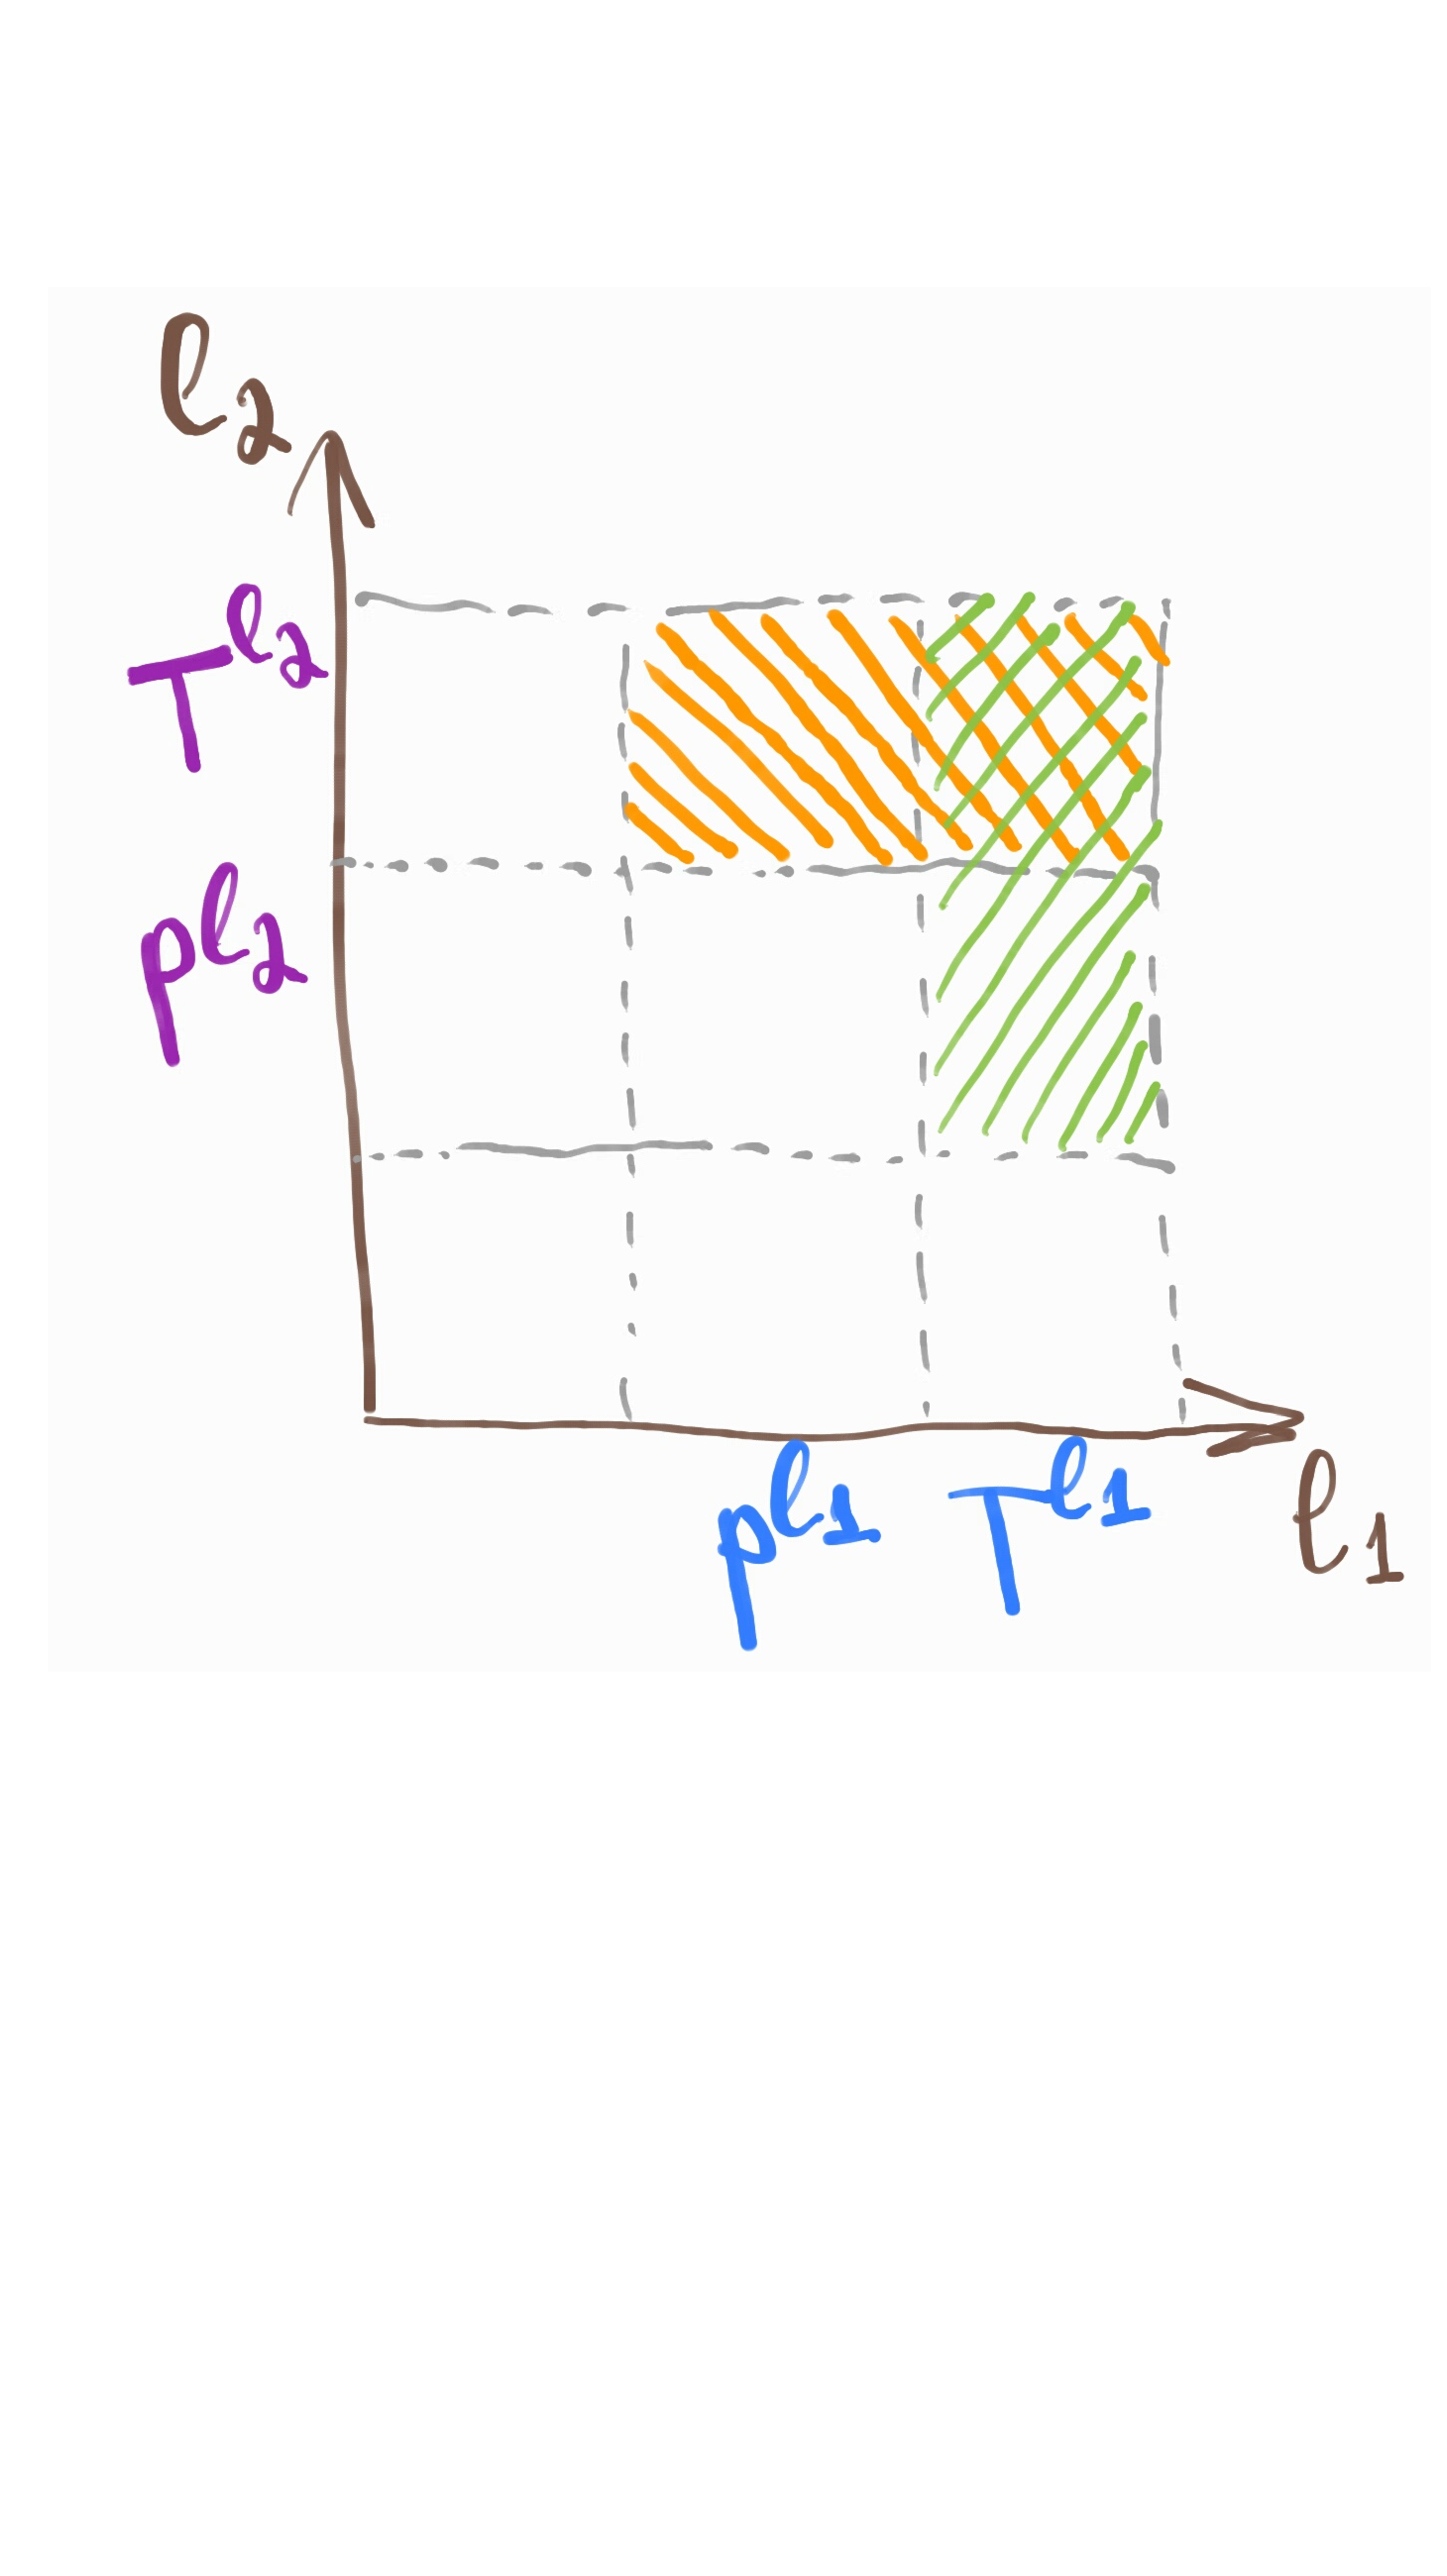
\includegraphics[width=0.6\textwidth]{TnP_sketch}
%  \caption[Sketch of the TnP method.]{Sketch of the TnP method. Phase space of efficiencies of two leptons is shown. The selection becomes tighter along the axes. Symbols $P^{l1}$ and $T^{l2}$ refer to efficiencies of the first lepton to pass the probe selection and of the second lepton to pass the tag selection respectively. The area, when probe leptons also pass tag selection, is coloured by both green and orange and is located at the upper right cell. This are should be removed as it leads to double counting of the number of pairs.}
%  \label{TnP_sketch}
%\end{figure}
%
%\noindent where the naming convention is as follows: $\epsilon_{1T}$ refers to the efficiency of the first lepton passing tag selection, $\epsilon_{2P}$ refers to the efficiency of the second lepton passing probe selection, etc. 
%
%At times, the probe can also pass a relatively tight selection of a tag. In this case, a double counting occurs. The extra pairs need to be removed. On the Fig. \ref{TnP_sketch} the area that contains double counted pairs is at the top right corner and corresponds to the di-lepton efficiency $\epsilon_{1T}\epsilon_{2T}$, this area is subtracted in the calculation of the $\epsilon_{HLT}$.

In addition, some HLT paths contained the DZ requirement, while others did not. Therefore, one needs to estimate additional efficiency related to the DZ selection and derive the corresponding SFs. The DZ scale factor calculation is very similar to estimation of efficiencies of all other sorts: the numerator contains events that pass the DZ requirement and the denominator is equal to the number of events that pass the selection without DZ requirement. Exactly the same procedure is applied to derive tracker, ID, and ISO SFs. Analysis specific figures will be shown in the data analysis chapter. 

\subsubsection{b tagging efficiency}\label{sec:b_tagging}

Scale factors also need to be derived for b jets. Tracker misalignment and the imperfect knowledge of the hadronization process of the b quark are the factors that lead to data-MC discrepancies. Additionally, the Strip tracker had known inefficiencies during 2016 data taking, which resulted in poor b tagging performance: lower efficiency to tag real b jets and higher fake rate (incorrect mistagging of light jets or gluons as b jets). The SFs have been derived by the b tagging CMS POG for the use of the whole collaboration. These correction factors are measured using the ``true'' or ``generator'' (gen) flavor of the original quark in the MC. Based on that, the b tagging weight is assigned to the particle level jet that is matched to the reconstruction level jet. SFs are provided in $p_T$ and $\eta$ slices to make the b tagging efficiency more uniform across the whole kinematic phase space. Further, MC events are reweighed using the combined weights from all jets present in the events. 

In this measurement, the data analysis is performed with b jets tagged by the cMVAv2 (CMVA) algorithm. The $t\bar{t}$ process containing top and anti-top quark decays is used to determine the b tagging weights. The CMVA discriminant should be above a certain threshold for b jets to be considered originating from the b quarks. The threshold is chosen to correspond to the medium working point of the algorithm defined such that the misidentification rate for light-quark and gluon jets is about 1$\%$.  The b jet tagging efficiency for this WP is about 66$\%$.


\section{Datasets and Trigger Paths}\label{sec:data_and_trigger}

The proton-proton collision data recorded by CMS is split into "eras", which are labelled using alphabetic letters A $\rightarrow $ H. Period A was dedicated to commissioning of the LHC for 2016 data taking. Periods from B to H were used for physics. Each era corresponds to a relatively stable period of the LHC conditions, such as the collision rate, the set of trigger menus, etc. Eras B to G were re-reconstructed at the end of 2016 to take advantage of the updated calibration of subsystems and the detector alignment. The data from the last era (H) was re-reconstructed during data-taking itself. 

Dozens of datasets (Primary Datasets or PDs) are recorded and stored by the CMS and its computing centers. The data that is analysed in this thesis belongs to ``Dimuon''(``DoubleMuon'') or ``Dielectron''(``DoubleEG'') datasets. This naming practice comes from the fact that to select these PDs, the HLT paths with two prompt muons or electrons were used. 

The name of the trigger paths (L1 in this case) reflects the number of leptons selected by a given trigger, the type of the lepton(s), following by the minimal $p_T$ requirement(s) on the lepton candidate(s). If two leptons are present, their $p_T$'s are referred to as $p_T$'s of the leading and subleading(trailing) lepton (another common naming is two ``legs''). If the suffixes ``Iso'' or ``Id'' (or ``ID'') are present, it indicates that the isolation or identification requirements respectively have been also applied. The label ``DZ'' or ``dz'' is an additional requirement on the spatial compatibility along the z axis between the lepton candidates and the PV location. Abbreviations VVL and VL refer to ``very very loose'' and ``very loose'' selections respectively. Their exact definition may vary, but the important point is that this selection does reject some clear fakes, while is still loose enough to leave enough statistics for offline analysers. 

\begin{table}[H]
\caption{Triggers for dimuon and dielectron channels both at L1 and HLT levels.}
\label{tab:trgs2015}
\begin{center}
\scalebox{0.75}{
\begin{tabular}{|m{9em}|m{5cm}|m{10cm}|} \hline%\hline
 Channel                    & L1 Paths                 & HLT Paths                                                         \\ \hline
``Dimuon'' Z$(\Pgm\Pgm)$~\Znn \HBB       & {\texttt L1\_SingleMu20}          & {\texttt HLT\_Mu17\_TrkIsoVVL\_Mu8\_TrkIsoVVL\_v* OR}                    \\
                              & { }                        & {\texttt HLT\_Mu17\_TrkIsoVVL\_TkMu8\_TrkIsoVVL\_v* OR}         \\
                              & { }                        & {\texttt HLT\_Mu17\_TrkIsoVVL\_Mu8\_TrkIsoVVL\_DZ\_v* OR}         \\
                              & { }                        & {\texttt HLT\_Mu17\_TrkIsoVVL\_TkMu8\_TrkIsoVVL\_DZ\_v*}         \\ \hline
``Dielectron'' Z$(\Pe\Pe)$~\Znn \HBB         & {\texttt L1\_SingleEG30      OR}  & {\texttt HLT\_Ele23\_Ele12\_CaloIdL\_TrackIdL\_IsoVL\_DZ } \\
                              & {\texttt L1\_SingleIsoEG22er OR}  & {  }         \\
                              & {\texttt L1\_SingleIsoEG24   OR}  & {  }         \\
                              & {\texttt L1\_DoubleEG\_15\_10  }  & {  }         \\ \hline
%\hline%\hline
\end{tabular}
			}
\end{center}
\end{table}


A simplified version of the PF event reconstruction sequence is performed at the HLT level. This sequence is based only on the regional track finding and fitting, relying on the muon and electron candidates found by L1 trigger. The HLT paths refer to triggers that select events where one or two leptons that pass certain selection criteria are present. HLT muons (abbreviated to ``Mu'') are formed by propagating the L1 track inwards to the inner tracker, or by starting from an inner track and projecting it to the outer tracker. HLT tracker muons (abbreviated to ``TkMu'') are reconstructed using the muon tracking procedure discussed in the Section \ref{sec:muon_track_reconstruction}. The HLT electrons are reconstructed using L1 seeds and checking their compatibility with the energy deposits in the ECAL. If the ID selection is applied on the track, the candidate name contains the suffix ``TrackId''. If the ID is applied on the ECAL energy cluster parameters, the name of the path contains ``CaloId''.


In the next chapter, there will be a thorough discussion of the physics analysis of the data produced by the LHC and collected with the CMS detector that have been used to perform the measurement of the double Higgs boson decays.


